\documentclass[12pt]{article}

\pagestyle{empty}
\setlength{\topmargin}{0in}
\setlength{\headheight}{0in}
\setlength{\topsep}{0in}
\setlength{\textheight}{9in}
\setlength{\oddsidemargin}{0in}
\setlength{\evensidemargin}{0in}
\setlength{\textwidth}{6.5in}

\usepackage{palatino,graphics,amsmath,amssymb,enumitem}

\newcommand{\ds}{\displaystyle}
\newcommand{\vs}[1]{\vspace{#1in}}
\renewcommand{\vss}[1]{\vspace*{#1in}}
\newcommand{\bvec}{{\mathbf b}}
\newcommand{\cvec}{{\mathbf c}}
\newcommand{\dvec}{{\mathbf d}}
\newcommand{\evec}{{\mathbf e}}
\newcommand{\fvec}{{\mathbf f}}
\newcommand{\qvec}{{\mathbf q}}
\newcommand{\uvec}{{\mathbf u}}
\newcommand{\vvec}{{\mathbf v}}
\newcommand{\wvec}{{\mathbf w}}
\newcommand{\xvec}{{\mathbf x}}
\newcommand{\yvec}{{\mathbf y}}
\newcommand{\zvec}{{\mathbf y}}
\newcommand{\zerovec}{{\mathbf 0}}
\newcommand{\real}{{\mathbb R}}
\newcommand{\twovec}[2]{\left[\begin{array}{r}#1 \\ #2
    \end{array}\right]}
\newcommand{\ctwovec}[2]{\left[\begin{array}{c}#1 \\ #2
   \end{array}\right]}
\newcommand{\threevec}[3]{\left[\begin{array}{r}#1 \\ #2 \\ #3
  \end{array}\right]}
\newcommand{\cthreevec}[3]{\left[\begin{array}{c}#1 \\ #2 \\ #3
    \end{array}\right]}
\newcommand{\fourvec}[4]{\left[\begin{array}{r}#1 \\ #2 \\ #3 \\ #4
    \end{array}\right]}
\newcommand{\cfourvec}[4]{\left[\begin{array}{c}#1 \\ #2 \\ #3 \\ #4
    \end{array}\right]}
\newcommand{\mattwo}[4]{\left[\begin{array}{rr}#1 & #2 \\ #3 & #4 \\ \end{array}\right]}
\renewcommand{\span}[1]{\text{Span}\{#1\}}
\newcommand{\bcal}{{\cal B}}
\newcommand{\ccal}{{\cal C}}
\newcommand{\scal}{{\cal S}}
\newcommand{\wcal}{{\cal W}}
\newcommand{\ecal}{{\cal E}}
\newcommand{\coords}[2]{\left\{#1\right\}_{#2}}
\newcommand{\gray}[1]{\color{gray}{#1}}
\newcommand{\lgray}[1]{\color{lightgray}{#1}}
\newcommand{\rank}{\text{rank}}
\newcommand{\col}{\text{Col}}
\newcommand{\nul}{\text{Nul}}

\begin{document}

\noindent
{\bf Mathematics 227} \\ 
{\bf Review}

\begin{enumerate}
\item Consider the matrix
  $$
  A =
  \left[
    \begin{array}{cc}
      0 & 2 \\
      1 & 1 \\
    \end{array}
  \right].
  $$

  What is the characteristic equation of $A$?

  \vs{1}
  What are the eigenvalues of $A$?

  \vs{1}
  Find a basis for the eigenspaces.

  \vs{1.5}
\item Suppose that $A$ is a $2\times2$ matrix having eigenvectors
  $\vvec_1=\twovec32$ and $\vvec_2=\twovec21$ and associated eigenvalues
  $\lambda_1 = -2$ and $\lambda_2 = 4$.  Find $A\twovec10$ and
  $A^2\twovec10$.  

  \newpage

\item Suppose that $\lambda = 0$ is an eigenvalue of $A$.  What does
  this say about the invertibility of $A$?

  \vs{1}
  If $A$ is invertible and $\lambda$ is an eigenvalue, explain why
  $\frac1\lambda$ is an eigenvalue of $A^{-1}$.

  \vs{1}

\item Consider the matrix
  $A =
  \left[
    \begin{array}{cc}
      -15 & 26 \\
      -10 & 17 \\
    \end{array}
  \right]
  $
  Identify the type of dynamical system this matrix defines and sketch
  a phase portrait.

  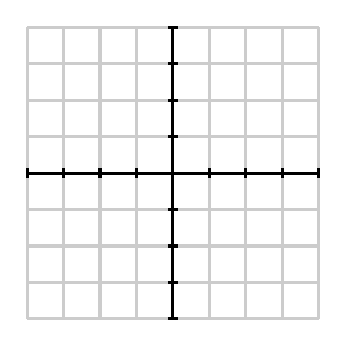
\includegraphics{empty.eps}

\item Consider the matrix
  $
  A =
  \left[
    \begin{array}{ccc}
      -1 & 0 & 2 \\
      -2 & -2 & -4 \\
      0 & 0 & -2 \\
    \end{array}
  \right]
  $.
  Can you find a basis for $\real^3$ consisting of eigenvectors of $A$?

  \newpage
\item The populations of two species $R$ and $S$ in year $k$ are
  denoted by $R_k$ and $S_k$.  Their populations in the following year
  are given by
  $$
  \begin{aligned}
    R_{k+1} & = R_k + S_k \\
    S_{k+1} & = 0.5R_k+1.5S_k. \\
  \end{aligned}
  $$
  Denote the state vector $\xvec_k=\twovec{R_k}{S_k}$.  Find the
  matrix $A$ such that $\xvec_{k+1}=A\xvec_k$.

  \vs{1}
  Identify the type of this dynamical system and sketch a phase
  portrait.

  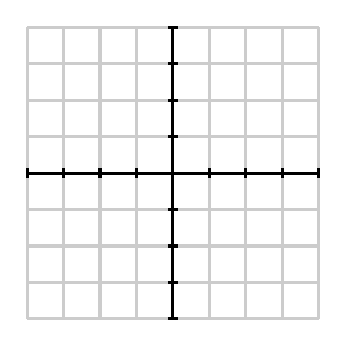
\includegraphics{empty.eps}

  After a very long time, what is the ratio of the populations
  $R_k/S_k$ and what is the growth rate of the populations?

  \vs{1}
\item Consider the matrix
  $A = 
  \left[
    \begin{array}{ccc}
      0.2 & 0.2 & 0.1 \\
      0.5 & 0.8 & 0.2 \\
      0.3 & 0.0 & 0.7 \\
    \end{array}
  \right]
  $.

  Find the eigenvalues of $A$.

  \vs{1}
  \newpage
  Find a steady-state vector $\qvec$.

  \vs{1}
  What happens to a Markov chain that begins with the initial state
  vector $\xvec_0 =\threevec{0.5}0{0.5}$?  

  \vs{1}
  Does the Perron-Frobenius theorem apply to this Markov chain?
  Explain why or why not.

  
  



\end{enumerate}


\end{document}
